\section{بخش دوم: تخمین پس‌زمینه با عملگر \lr{Dilation}}

\begin{stepbox}
\field{هدف این بخش (بخش ۲)}{
استفاده از عملگر بسط دادن (\lr{Dilation}) در حوزه پیوسته با پنجره‌های مستطیلی در ابعاد $41\times41$، $51\times51$ و $61\times61$ برای تخمین زدن و استخراجِ نقشه‌ی پس‌زمینه (سایه). همچنین تنظیم مقادیرِ حاشیه‌های بیرون‌زده از تصویر بر روی مقدار صفر.
}
\end{stepbox}

\subsection{کد پیاده‌سازی و منطق آن}
برای این قسمت، نیازی به پیاده‌سازی دستیِ فیلتر نیست و از توابع بهینه‌شده‌ی کتابخانه \lr{OpenCV} بهره می‌بریم. قطعه کد کلیدیِ این بخش در زیر آورده شده است:

\begin{codebox}[\lr{Dilation Operation}]
\begin{lstlisting}[language=Python]
# Create a square kernel of ones
kernel = np.ones((k, k), np.uint8)

# Apply Dilation with zero padding at borders
dilated = cv2.dilate(img, kernel, borderType=cv2.BORDER_CONSTANT, borderValue=0)
\end{lstlisting}
\end{codebox}

\textbf{توضیح کد:}
ابتدا یک ماتریسِ همسایگی (\lr{Kernel}) با ابعاد خواسته‌شده (\lr{k} در \lr{k}) ساخته می‌شود که تمام درایه‌های آن یک است. سپس تابع \lr{\texttt{cv2.dilate}} این پنجره را روی تصویر حرکت می‌دهد. برای رعایت شرطِ مساله مبنی بر صفر در نظر گرفتن حاشیه‌ها، از پارامترهای \lr{\texttt{borderType=cv2.BORDER\_CONSTANT}} و \lr{\texttt{borderValue=0}} استفاده شده است تا اگر پنجره از کادر تصویر خارج شد، مقادیر بیرون‌زده با صفر پر شوند.

\subsection{خروجی‌های تصویری و تحلیل دقیق آن‌ها}
خروجی اعمال این فیلتر با سه ابعاد مختلف در شکل \ref{fig:part2_dilation} نشان داده شده است.

\begin{figure}[h!]
    \centering
    \begin{subfigure}{0.31\textwidth}
        \centering
        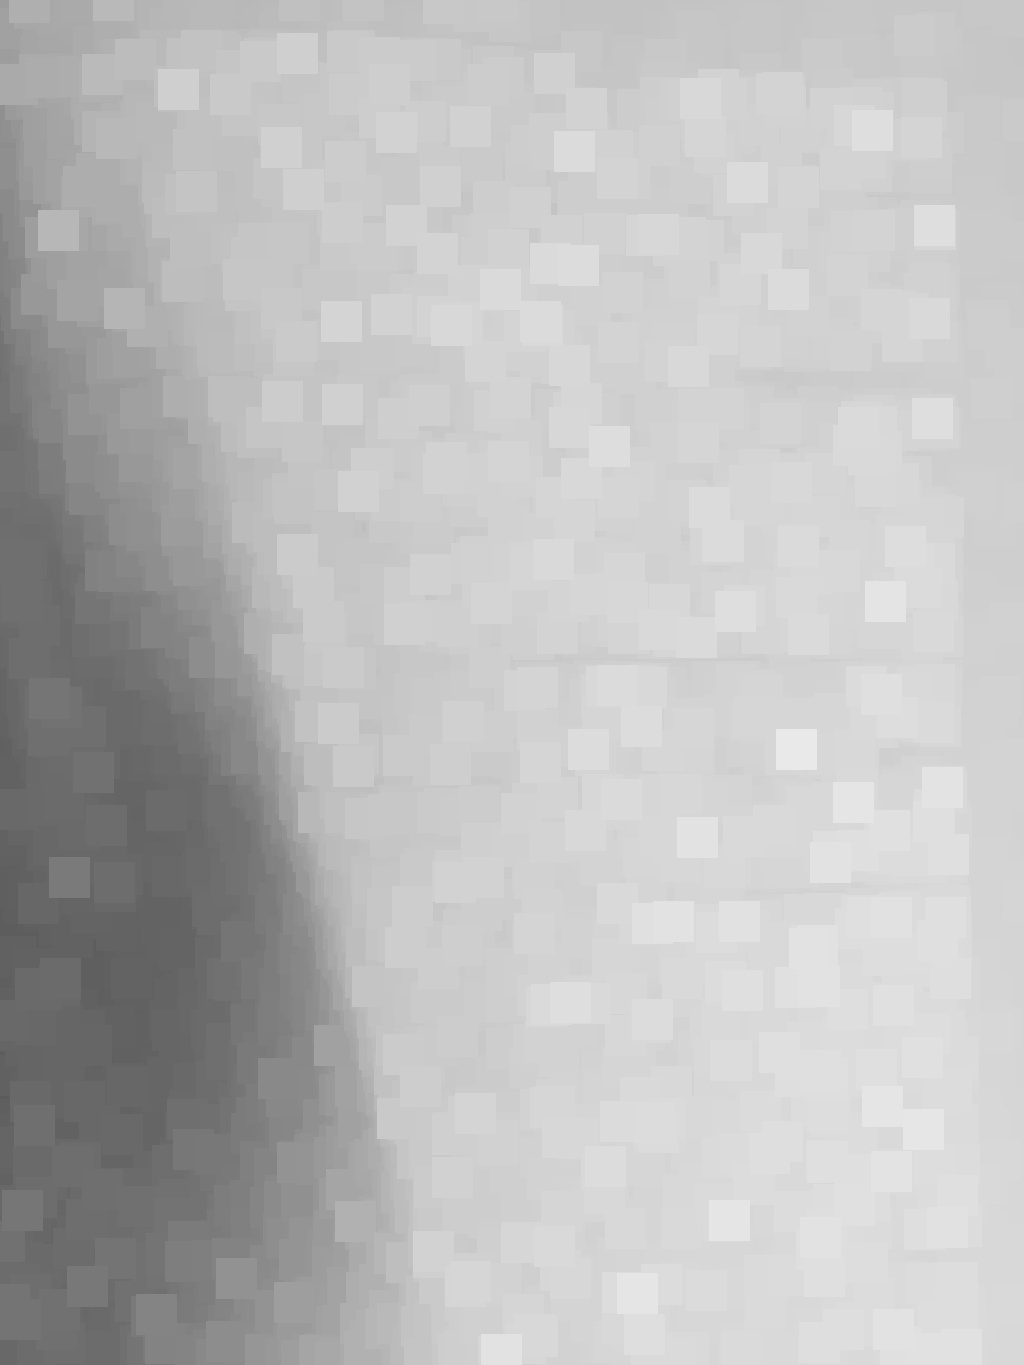
\includegraphics[width=\linewidth]{images/dilated_41x41.jpg}
        \caption{پنجره $41\times41$}
    \end{subfigure}
    \hfill
    \begin{subfigure}{0.31\textwidth}
        \centering
        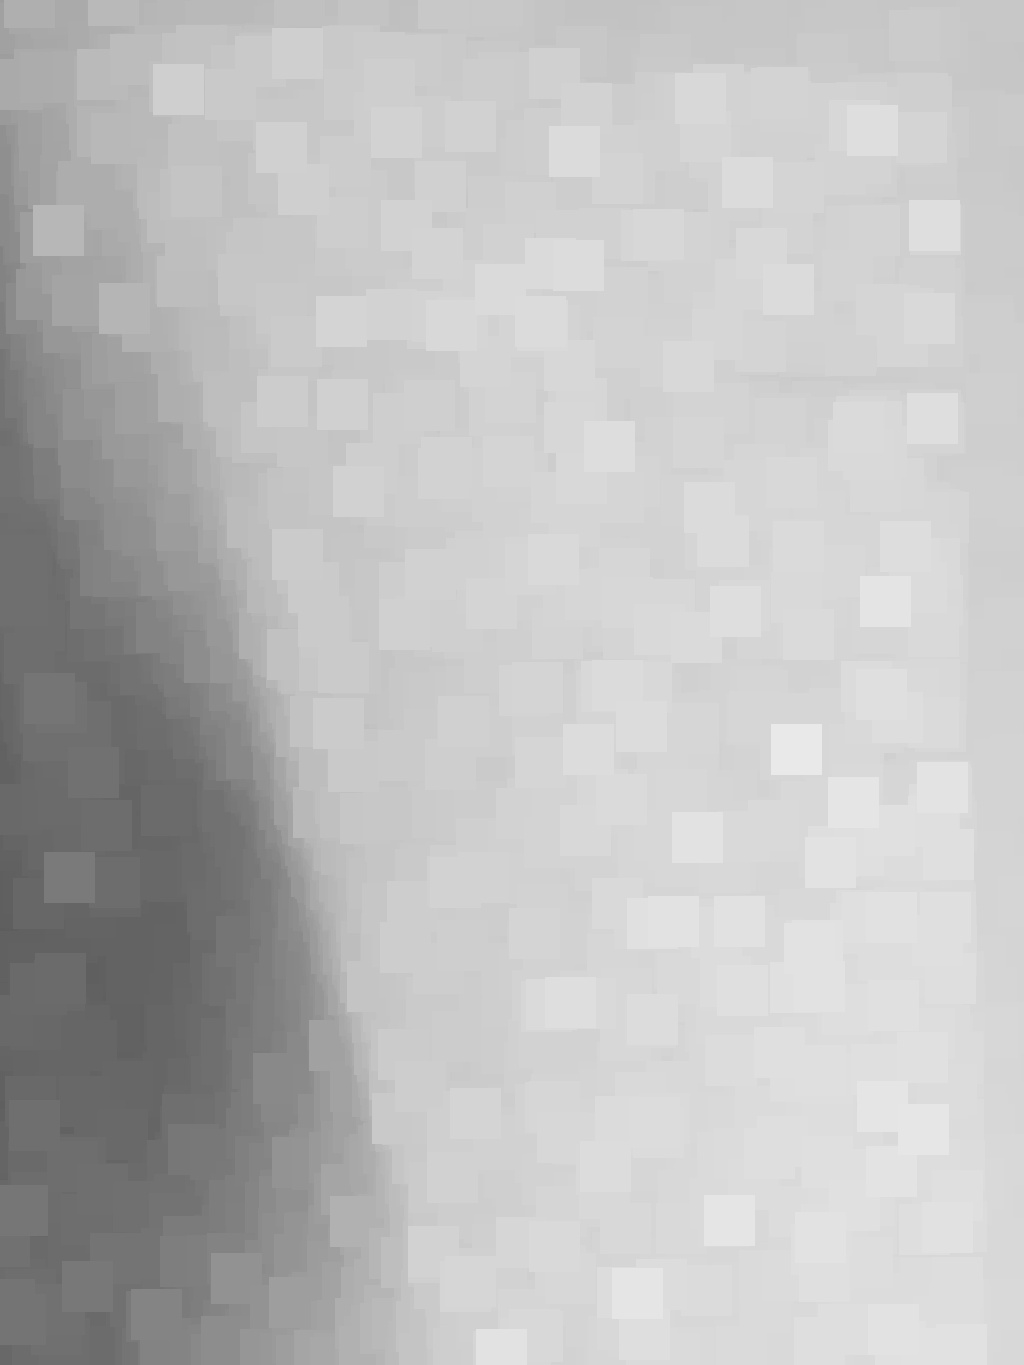
\includegraphics[width=\linewidth]{images/dilated_51x51.jpg}
        \caption{پنجره $51\times51$}
    \end{subfigure}
    \hfill
    \begin{subfigure}{0.31\textwidth}
        \centering
        
\includegraphics[width=\linewidth]{images/dilated_61x61.jpg}
        \caption{پنجره $61\times61$}
    \end{subfigure}
    \caption{نقشه تخمینی پس‌زمینه با اعمال عملگر \lr{Dilation}}
    \label{fig:part2_dilation}
\end{figure}

\textbf{کالبدشکافی منطق \lr{Dilation} و تحلیل خروجی‌ها:}
در پردازش تصویرِ سطح خاکستری (\lr{Grayscale})، عملگر \lr{Dilation} به عنوان یک فیلترِ «ماکزیمم‌گیر» عمل می‌کند. این فیلتر در هر نقطه‌ای که قرار می‌گیرد، روشن‌ترین پیکسل در آن همسایگی را انتخاب کرده و جایگزینِ پیکسلِ مرکزی می‌کند. 
از آنجایی که در تصویر ما حروف متنی تاریک و پس‌زمینه روشن است، این عملگر در واقع بخش‌های تیره (متن) را پاک کرده و آن‌ها را با روشناییِ پس‌زمینه پر می‌کند. به همین دلیل خروجی‌ها شبیهِ به نقشه خالصی از نورپردازیِ محیط (تاریک در چپ و روشن در راست) شده‌اند و حروف متنی از بین رفته‌اند.

\subsection{پاسخ به سوالات تمرین}
\textbf{خروجی این سه حالت چه تفاوتی با یکدیگر دارند؟} \\
هرچه ابعاد پنجره‌ی مستطیلی بزرگ‌تر می‌شود، قدرتِ فیلتر در پاک کردنِ جزئیات تیره‌تر بیشتر می‌گردد. 
\begin{itemize}
    \item در پنجره‌ی $41\times41$، اگر دقت کنیم محدوده‌ی جستجو به اندازه‌ای نبوده که ضخامتِ کلماتِ درشت را کاملاً در بر بگیرد؛ لذا هاله‌ای از متون (به شکل خطوط افقی محو) همچنان در تصویر باقی مانده است.
    \item در پنجره‌ی $61\times61$، وسعتِ پنجره باعث شده تا حروف متنی به طور کامل‌تر محو شوند و نقشه‌ای یکنواخت‌تر از نورپردازی پس‌زمینه به دست بیاید. 
\end{itemize}
البته باید توجه داشت که بزرگ شدنِ بیش از حد پنجره در نواحیِ مرزیِ سایه (سمت چپ تصویر)، می‌تواند باعثِ نشت کردنِ روشنایی به داخل محدوده‌ی تاریک شده و هندسه‌ی واقعیِ سایه را مخدوش کند.